\chapter[Définition du sujet]{Définition du sujet}

\textit{Le présent chapitre a pour objectif de définir le sujet et son contexte d'étude. }

\section{Contexte du sujet}

Grâce au développement des techniques LiDAR et aux prises de vues aériennes et satellites, il est aujourd'hui facile de représenter la surface de la Terre. Cependant, dans le cas des zones urbaines, une modélisation plus avancée implique une phase de reconstruction 3D. \newline

Pour ce faire, on utilise un nuage de points, créé à partir de données LiDAR ou par reconstruction photogrammétrique. Une base de données est également associée au processus, et regroupe un ensemble des objets numériques représentant les bâtiments. Selon le type de modélisation envisagée, cette base est plus ou moins développée. L’étape de reconstruction consiste ensuite à associer une entité de la base de données à une partie du nuage de points, en se basant sur le principe de corrélation d’objets.\newline

\begin{figure}[!h]
	\begin{center}
		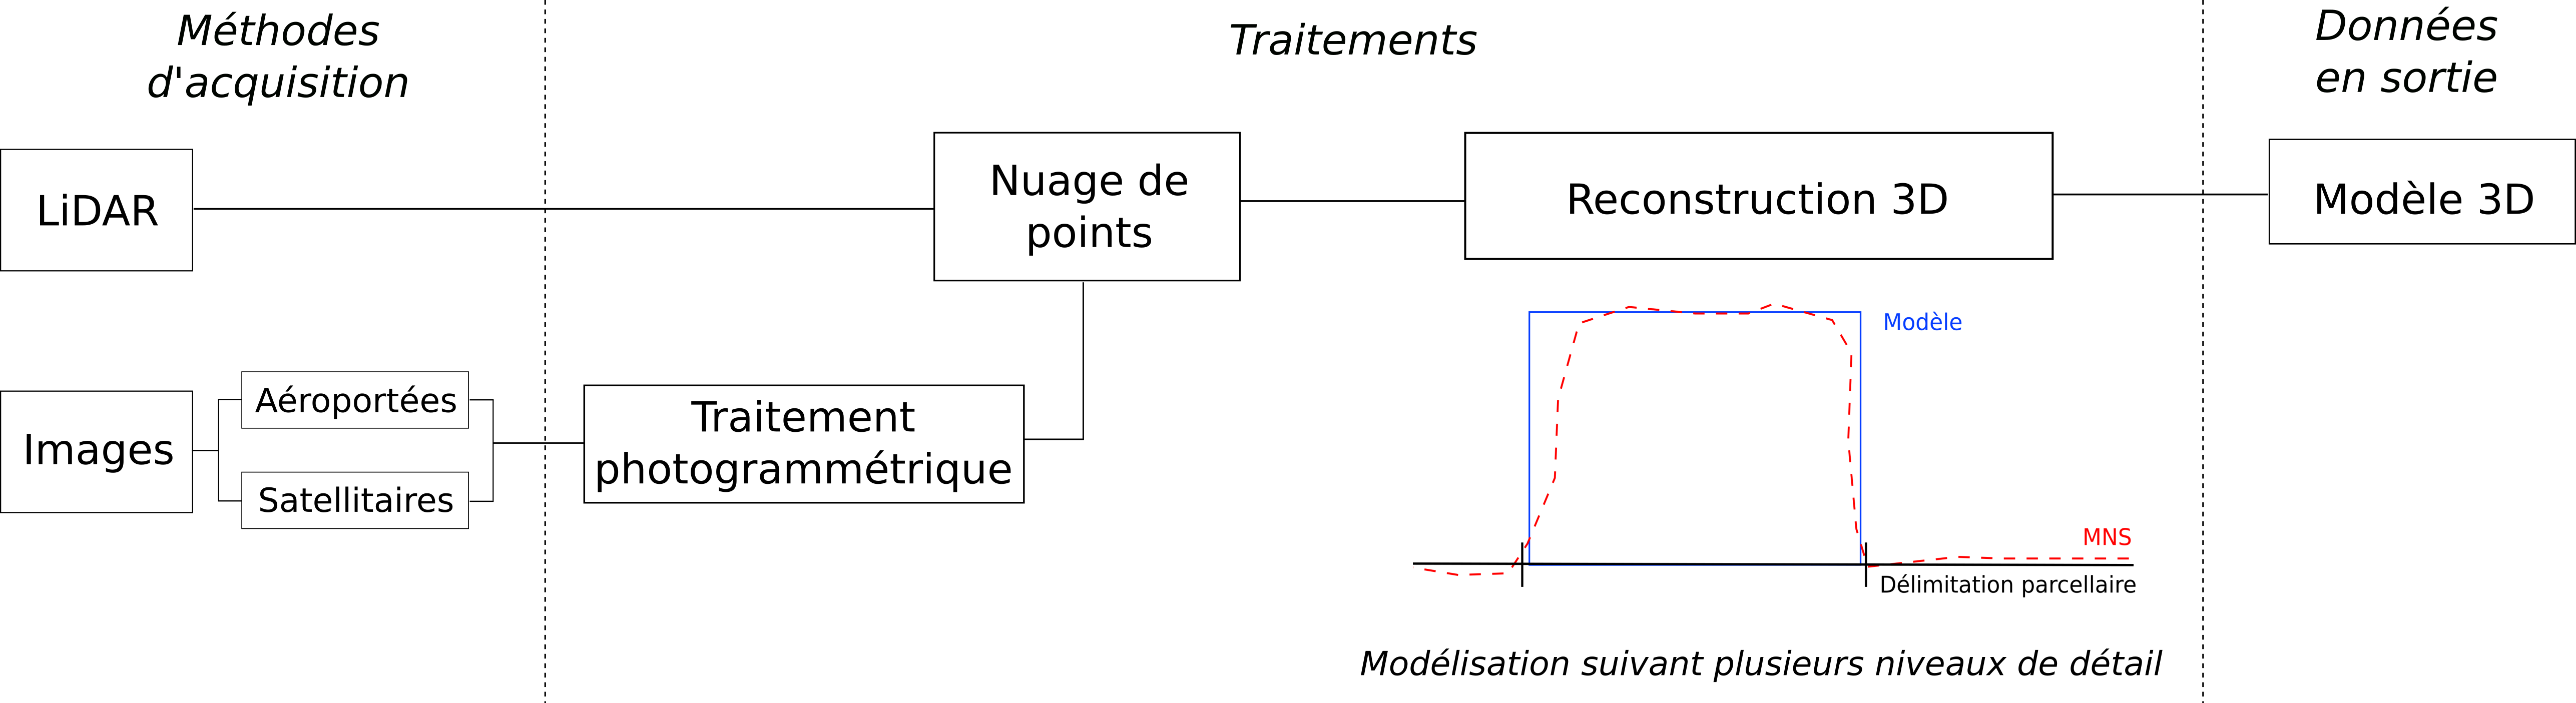
\includegraphics[scale=0.38]{Process_ini.png}  \\
		\caption[Chaîne de reconstruction 3D]{Chaîne de reconstruction 3D}
		\label{fig:recons3D}
	\end{center}
\end{figure}

\begin{figure}[!h]
	\begin{center}
		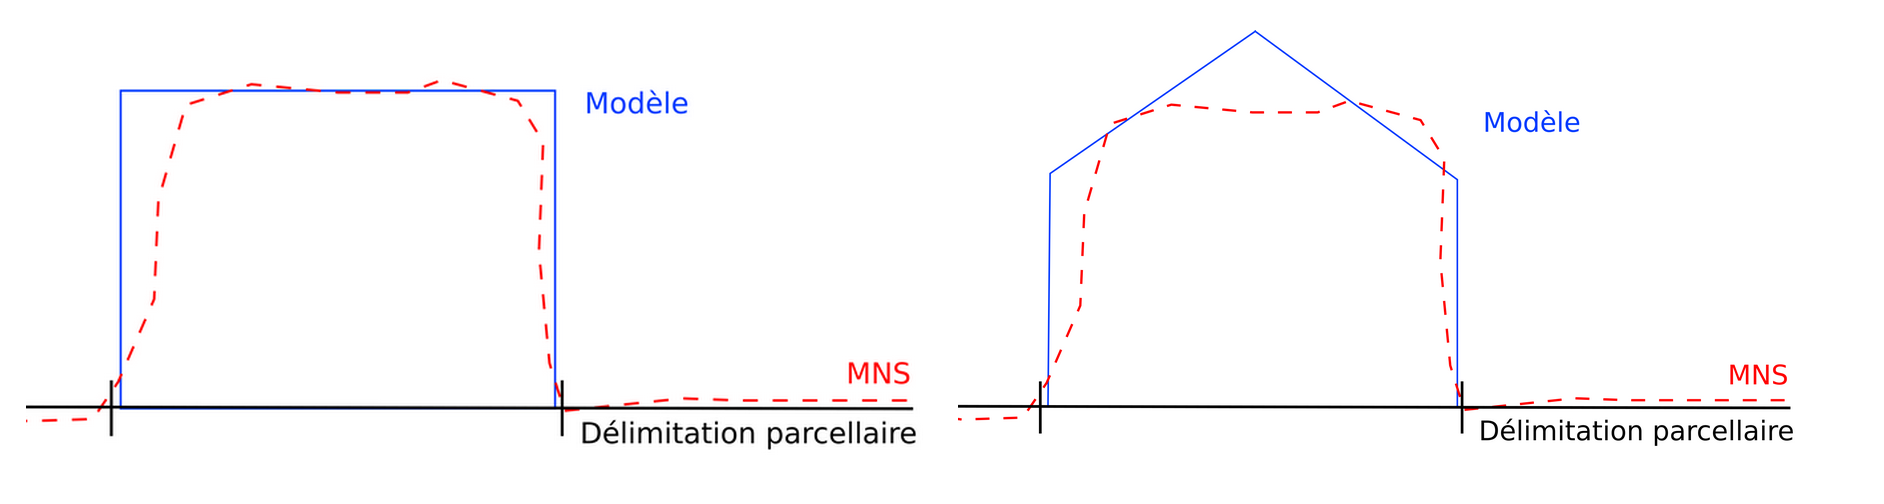
\includegraphics[scale=0.32]{Correlation.png}  \\
		\caption[Principe de corrélation d'objets]{Principe de corrélation d'objets}
		\label{fig:correlobj}
	\end{center}
\end{figure}

Selon le niveau de détail recherché, différents modèles sont possibles : Manhattan (= toits plats), Biplan (= toits pentus), Modélisation précise (à partir de la triangulation du MNS), … Plus le modèle est évolué, plus le niveau de détail est important mais plus la généralisation est compliquée et lourde à coder. \newline

\footnote{Sources : OGC CityGML Implementation Specification 1 (Research Center Karlsruhe)}
\begin{figure}[!h]
	\begin{center}
		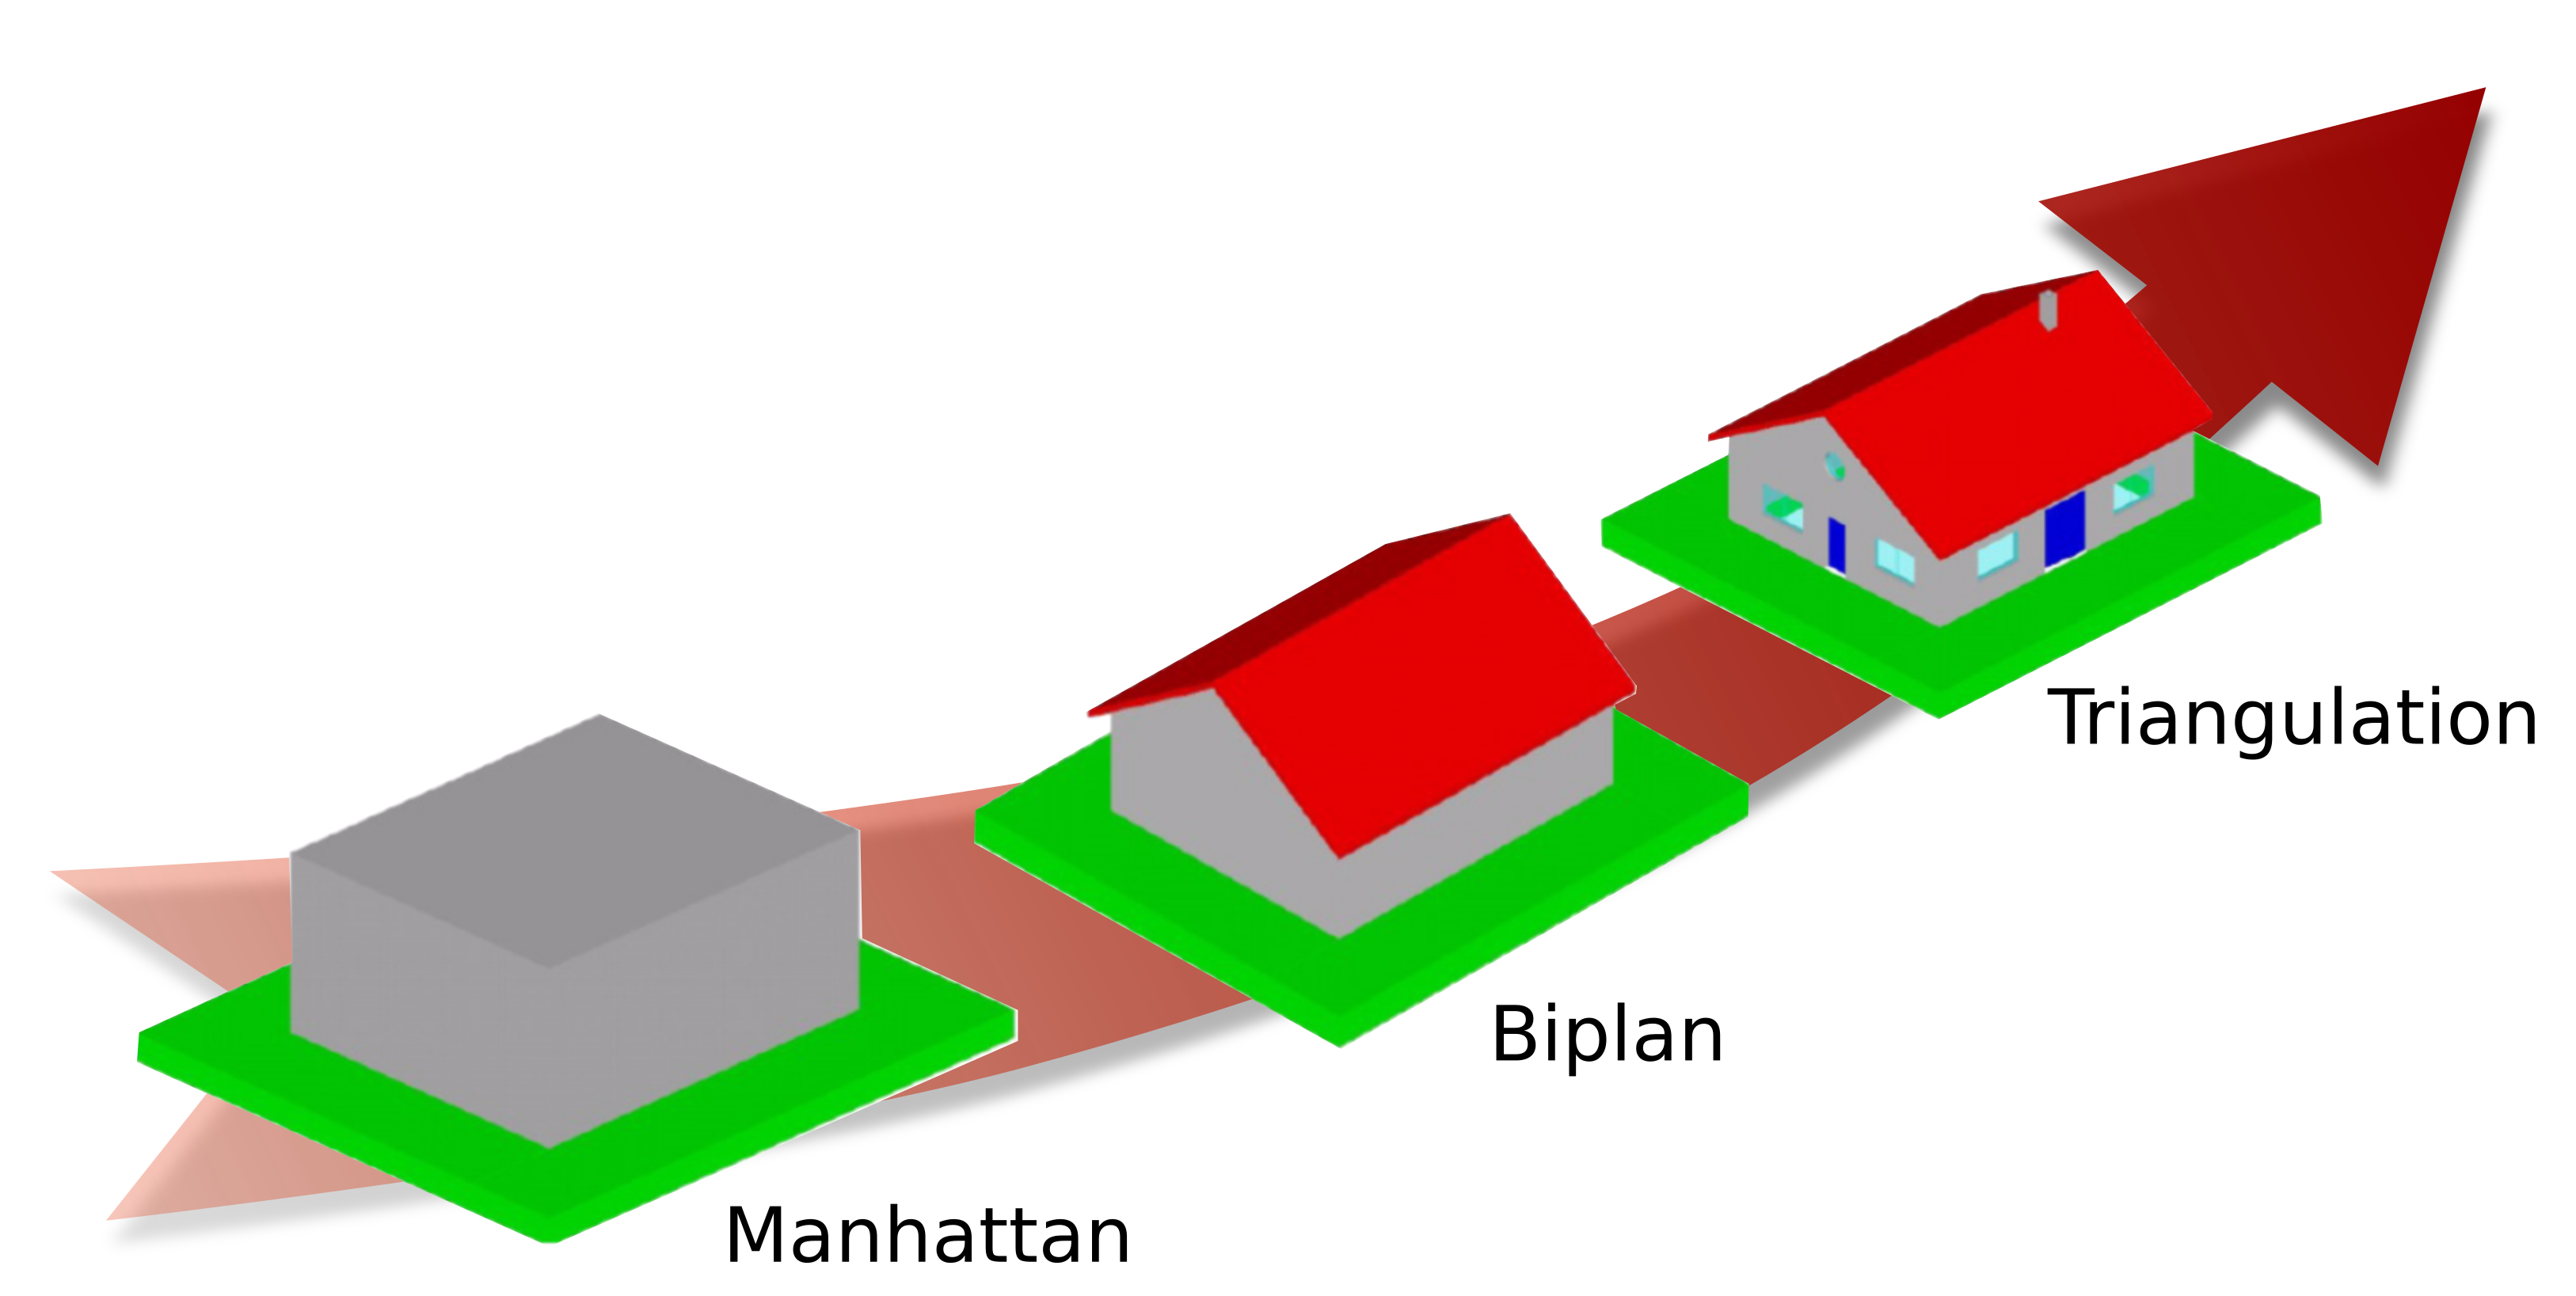
\includegraphics[scale=0.15]{Niveau_detail.png}  \\
		\caption[Impact du niveau de détail sur la modélisation]{Impact du niveau de détail sur la modélisation}
		\label{fig:LOD}
	\end{center}
\end{figure}

Aujourd'hui, les techniques de reconstruction automatiques ne sont pas opérationnelles. L’utilisateur doit intervenir pour corriger manuellement les erreurs, ce qui réduit le gain de temps envisagé par l'automatisation de la reconstruction. Pour faciliter ce retraitement, il est intéressant de pouvoir qualifier les erreurs commises. Pour cela, deux méthodes sont envisageables : la qualification avec des données de référence, et l’auto-qualification. \textbf{A PRECISER} \newline

En matière de reconstruction 3D, les laboratoires de l'IGN ont mis au point la base de donnée BATI-3D, permettant de naviguer dans des paysages urbains en 3 dimensions.\footnote{http://cours-fad-public.ensg.eu/mod/imscp/view.php?id=334} Le projet présenté ici s’inscrit dans le cadre des recherches du laboratoire Matis de l'IGN pour la reconstruction 3D des bâtiments à partir de MNS. L'objectif est d'associer un modèle prédéfini de bâtiment 3D à un objet numérique, reconstitué par le MNS et l’emprise au sol du bâtiment. \newline

\section{Problématique}

Pour détecter et caractériser les erreurs de reconstruction, l’équipe de recherche à mis en place une méthode d'auto-qualification. Ce processus passe par la réalisation d'une classification supervisée des entités reconstruites, afin de leur associer une classe d'erreur. \newline

Les différents types d'erreur sont ordonnées hiérarchiquement selon des classes, choisies en fonction du niveau de détail de la reconstruction. Ainsi, on peut définir une typologie des erreurs rencontrées (cf. annexe \ref{annexeerreurs}).\newline

L'objectif de cette méthode est d'évoluer vers une classification active. En effet, l'intervention d'un utilisateur permettrait de valider (ou non) les résultats de la classification, avant de relancer un processus de calcul.\newline
 
Le projet de développement présenté dans ce rapport propose donc de mettre en place un outil d'aide à la classification active. L'objectif est de réaliser une interface permettant à un utilisateur de valider un résultat de classification et d'annoter l'objet présenté. Pour cela, les objets d'intérêt (orthophotographie et emprise des bâtiments) doivent pouvoir être visualisés selon une hiérarchie à définir.\newline


\section{Analyse des besoins}

\subsection{Objectifs du projet}

Les principaux enjeux du projets sont liés à l'affichage et à la validation des résultats de la classification.

\begin{figure}[!h]
	\begin{center}
		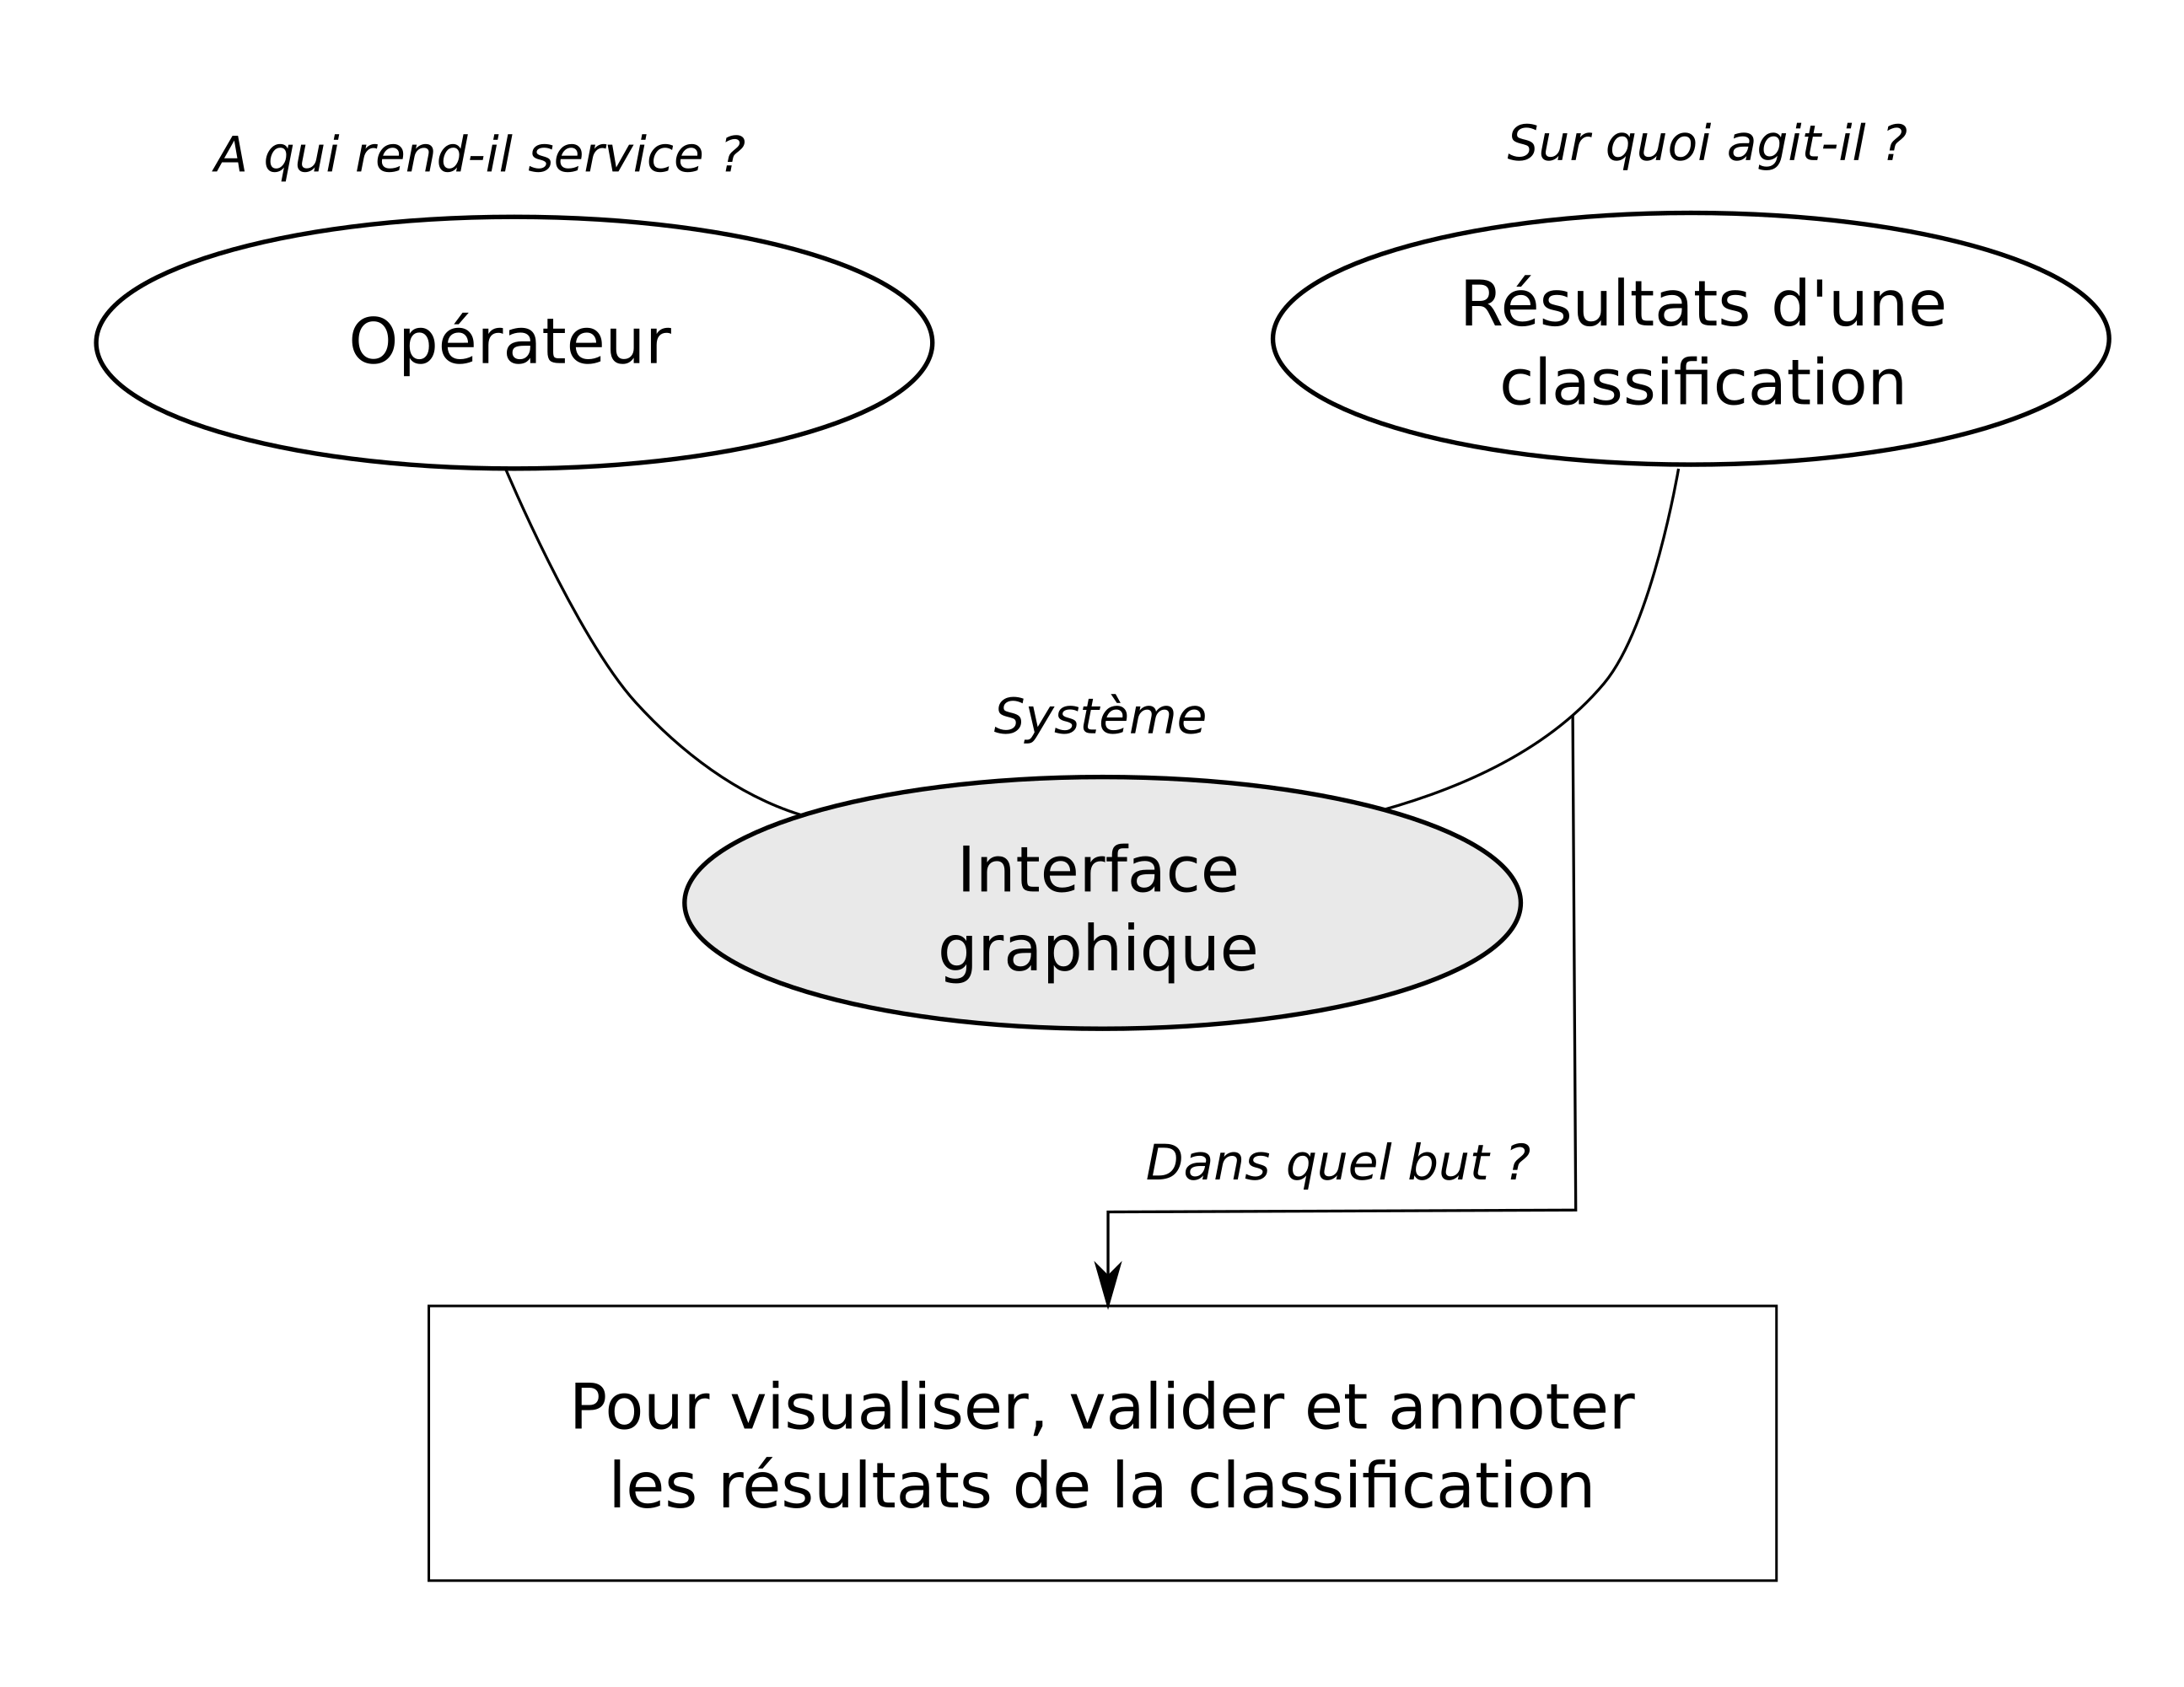
\includegraphics[scale=0.50]{Bete_corne.png}  \\
		\caption[Objectifs généraux du projet]{Objectifs généraux du projet}
		\label{fig:betecorne}
	\end{center}
\end{figure}

Dans un premier temps,ce projet s'adresse aux utilisateurs du processus de qualification des données de reconstruction 3D urbaine. Cependant, l'interface réalisée peut être amenée à évoluer et à servir de base de visualisation pour d'autres projets du laboratoire de l'IGN. 

\subsection{Calendrier prévisionnel}

(A revoir)